\chapter{引言}

本文主要讨论四土嘉绒语米亚罗话的音系。

\section{调查点概况}

四土嘉绒语米亚罗话主要分布在四川省阿坝藏族羌族自治州理县米亚罗镇（\tib{མྱག་ལོ།}，31°39′43″N 102°48′09″E）。

\begin{figure}[H]
\centering
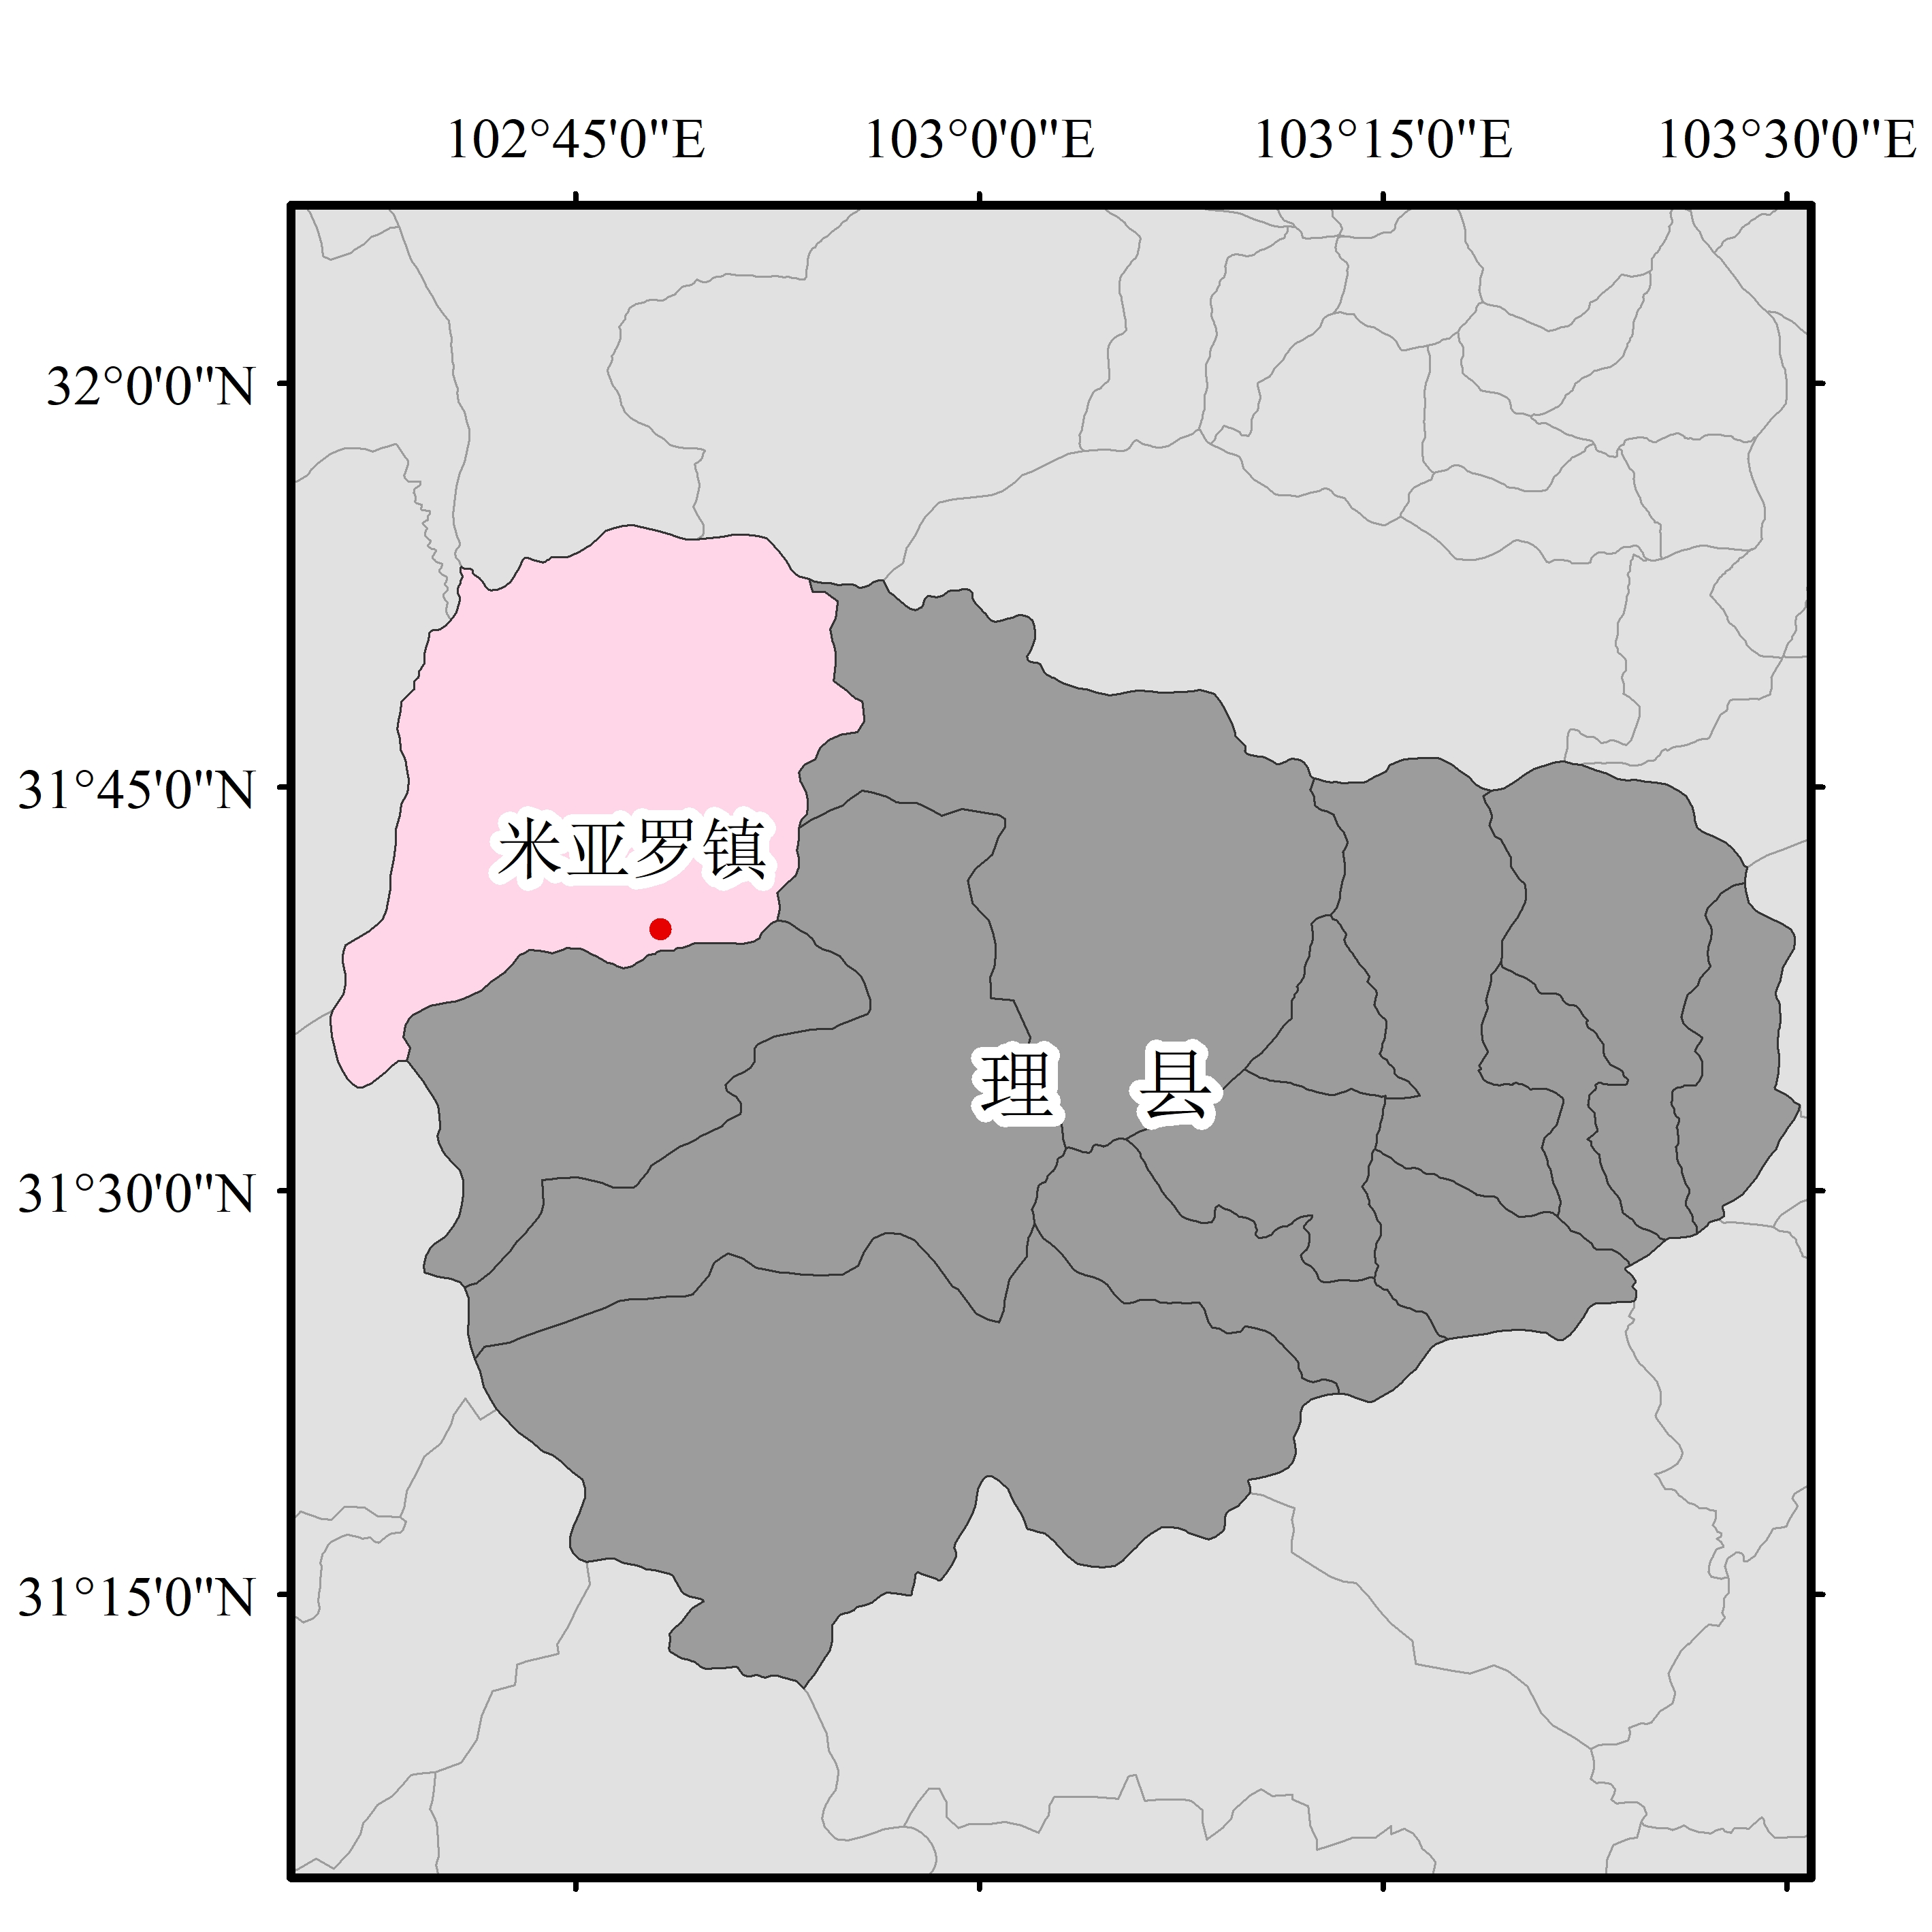
\includegraphics[width=0.8\textwidth]{img/LisCo.jpg}
\caption{米亚罗镇地理位置}
\label{myaglo}
\end{figure}

米亚罗镇位于理县西北部。唐贞观八年（634年）设北思县，治所北思城，即今米亚罗镇。后更名云山县。唐广德元年（763年）被吐蕃王国占领\cite[970-971]{xingzheng-2012}。清代，米亚罗镇为梭磨土司（\tib{སོ་མང།}）辖区，称为“柯宋（或扣苏）上四沟”\cite[79]{<<Li-Xian-Zhi->>-Bian-Zuan-Wei-Yuan-Hui-1997-gj}。梭磨土司，即“四土嘉绒语”之名中“四土”所代指的四个土司（卓克基土司、梭磨土司、松岗土司、党坝土司）之一\cite{sun2000parallelisms}。1928年将“柯宋（扣苏）”改为“来苏”，1951年设上来苏区自治政府，1954年设米亚罗区人民政府，1955年设米亚罗镇\cite[79]{<<Li-Xian-Zhi->>-Bian-Zuan-Wei-Yuan-Hui-1997-gj}。目前，米亚罗镇下辖一个社区和九个村：红叶社区、米亚罗村、胆杆村、斯博果村、八角碉村、大郎坝村、夹壁村、二古溪村、猛古村、吉柯村。

\begin{figure}[H]
\centering
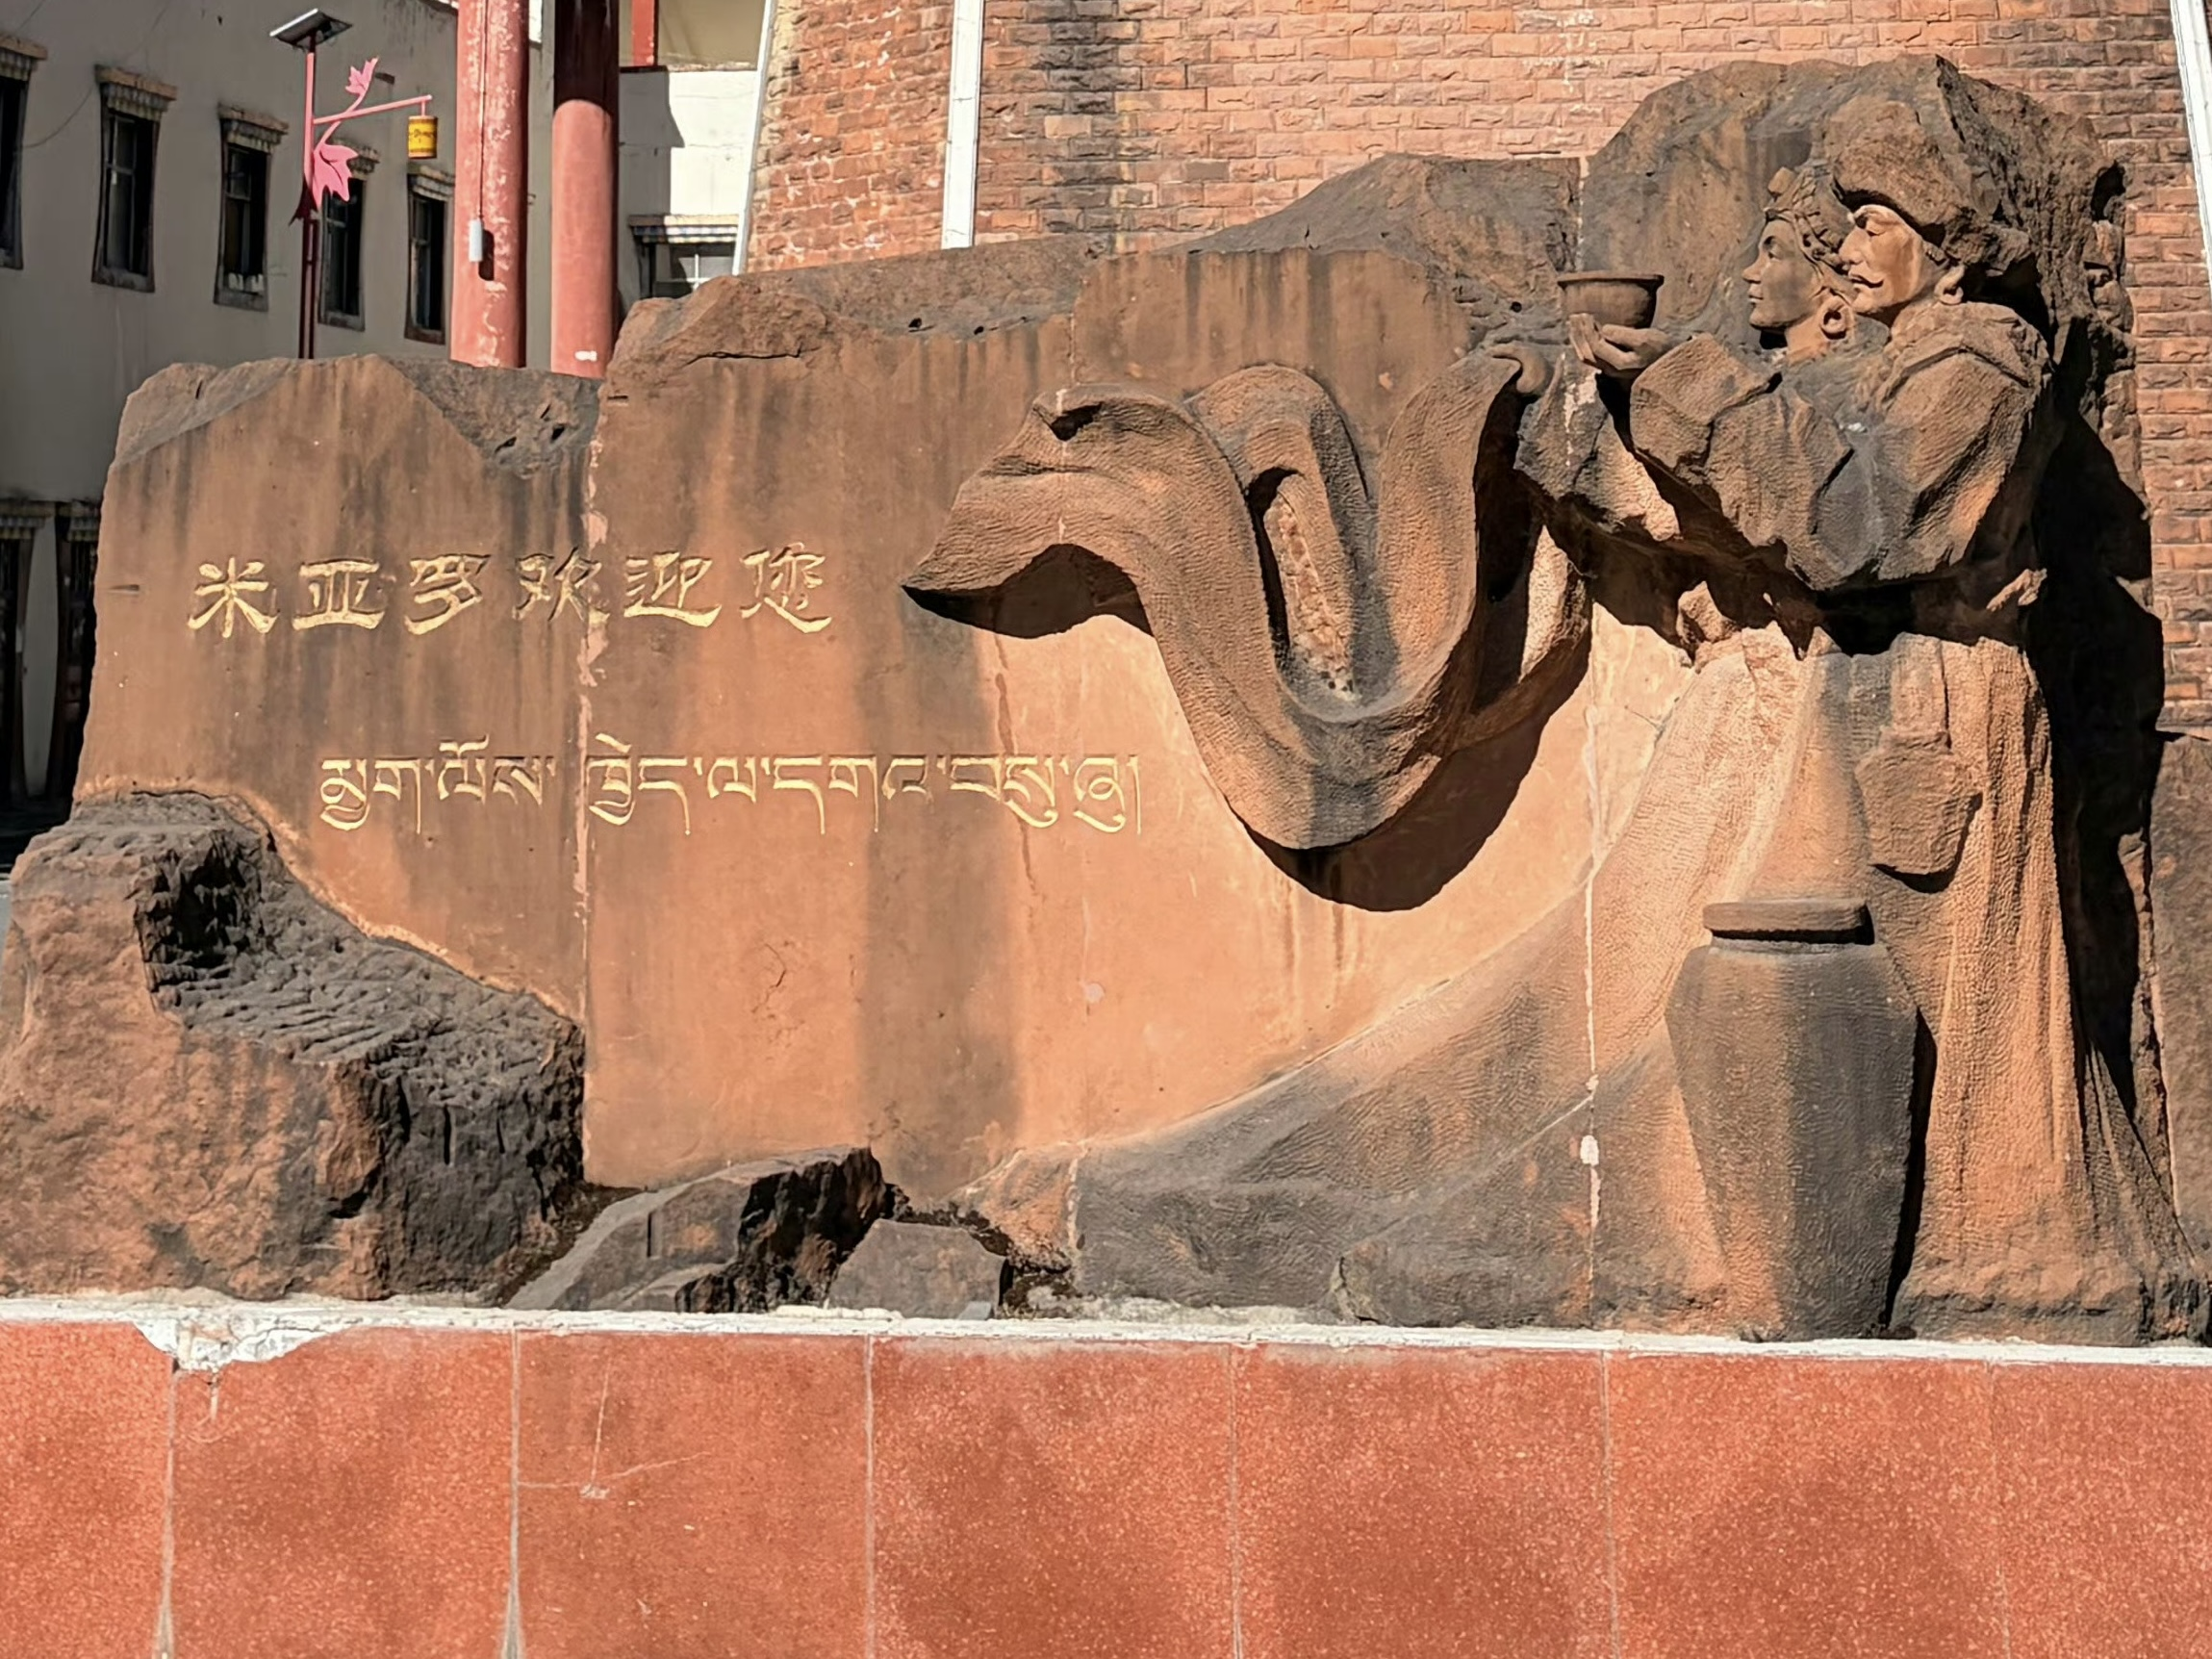
\includegraphics[width=0.8\textwidth]{img/miyaluo-pic2.jpg}
\caption{米亚罗（\tib{མྱག་ལོ།}）藏文转写}
\label{myaglopic}
\end{figure}

根据国家的民族识别工作，米亚罗镇的大多数四土嘉绒语母语者被识别为藏族。他们多数信仰藏传佛教宁玛派，不考虑语言因素，在生活习惯、文化上都接近藏族，自我认同也是藏族。除了藏族之外，米亚罗镇还存在部分汉族常住人口；作为旅游景区，米亚罗镇还有大量来自各地的游客。因而，米亚罗镇的四土嘉绒语主要和汉语普通话、西南官话存在接触，居民普遍存在四土嘉绒语和汉语的双语现象。此外，部分村落和寺庙也存在与藏语安多话（“草地话”）之间的接触。

现今，米亚罗镇的四土嘉绒语在各代人中均有保留。然而，虽然年轻一代的母语大多还是四土嘉绒语，但日常生活中的使用已大幅减少。在米亚罗镇及其下辖各村，大约有3000人正在使用四土嘉绒语米亚罗话。

\section{研究综述}

四土嘉绒语是汉藏语系嘉绒语组的一门独立语言，米亚罗话是四土嘉绒语的一个方言。

现代语言学意义上的“嘉绒语组”概念，最早由台湾语言学家孙天心提出。\textcite{sun2000parallelisms,sun2000stem}将当时的嘉绒语、霍尔巴—上寨语、拉坞戎语归类为藏缅语族羌语支内的一个独立语言支系。其中，“嘉绒语”下包括了四土话、茶堡话、四大坝话三个变体。向柏霖根据互通度将四大坝话拆分为草登话和日部话，认为“嘉绒语”有四土话、茶堡话、草登话、日部话四个方言\cite{Xiang2008,jacques2004phonologie}。近期的分类将嘉绒语组划分为东部嘉绒语组（也称核心嘉绒语组，包括四土嘉绒语、茶堡嘉绒语、草登嘉绒语、日部嘉绒语）和西部嘉绒语组（包括道孚语、绰斯甲语、西夏语）两支\cite{lai2020tangut}，分类树如下：

\begin{center}
    \begin{tikzpicture}
        \Tree
        [.嘉绒语组 
            [.东部嘉绒语组 
                [.四土嘉绒语 ]
                [.茶堡嘉绒语 ]
                [.草登嘉绒语 ]
                [.日部嘉绒语 ]
             ]
            [.西部嘉绒语组 
                [.道孚语 ]
                [.绰斯甲语 ]
                [.西夏语 ]
            ]
        ]
    \end{tikzpicture}
\end{center}

其中，四土嘉绒语是使用最广泛的嘉绒语组语言，分布在阿坝州的马尔康市、金川县、小金县、黑水县、理县、红原县、汶川县，以及甘孜州的丹巴县和雅安市的宝兴县\cite[411]{Lin-1993-cd}。四土嘉绒语同样是最早被记录的嘉绒语组语言。最早的文献记载是清代乾隆十五年（1750年）成书的《西蕃译语》，其中的《嘉绒译语》记载了740条四土嘉绒语词汇，采用藏文字母和汉字记音\cite{Gong2018-aw,Nie2010}。学术性报告则可追溯至19世纪末\cite{Von_Rosthorn1897-du}。早期的描写性著作包括\textcite{Jin1949-uh}对理县杂谷脑镇方言的研究，以及\textcite{Jin-1957-oe}对梭磨话的研究。随后，马尔康卓克基镇的卓克基话成为语言学研究的焦点，\textcite{Lin-1993-cd}提供了全面的语法，\textcite{Lin-2016-dr}提供了标注文本，\textcite{hsieh1999theoretical,lin2012no}分析了其音系，\textcite{Lin2000-jd,Nagano1984-tn,Wei2001-mw}分析了其动词形态。近年来，学界出版了四土嘉绒语其他方言的一些重要参考语法，包括\textcite{zhang2016phonologie,Zhang2020-ya}关于白湾话的参考语法、\textcite{prins2011web}关于脚木足话的著作、\textcite{Chang-Ye-2018-gb}对莫拉话的研究。

\begin{figure}[H]
\centering
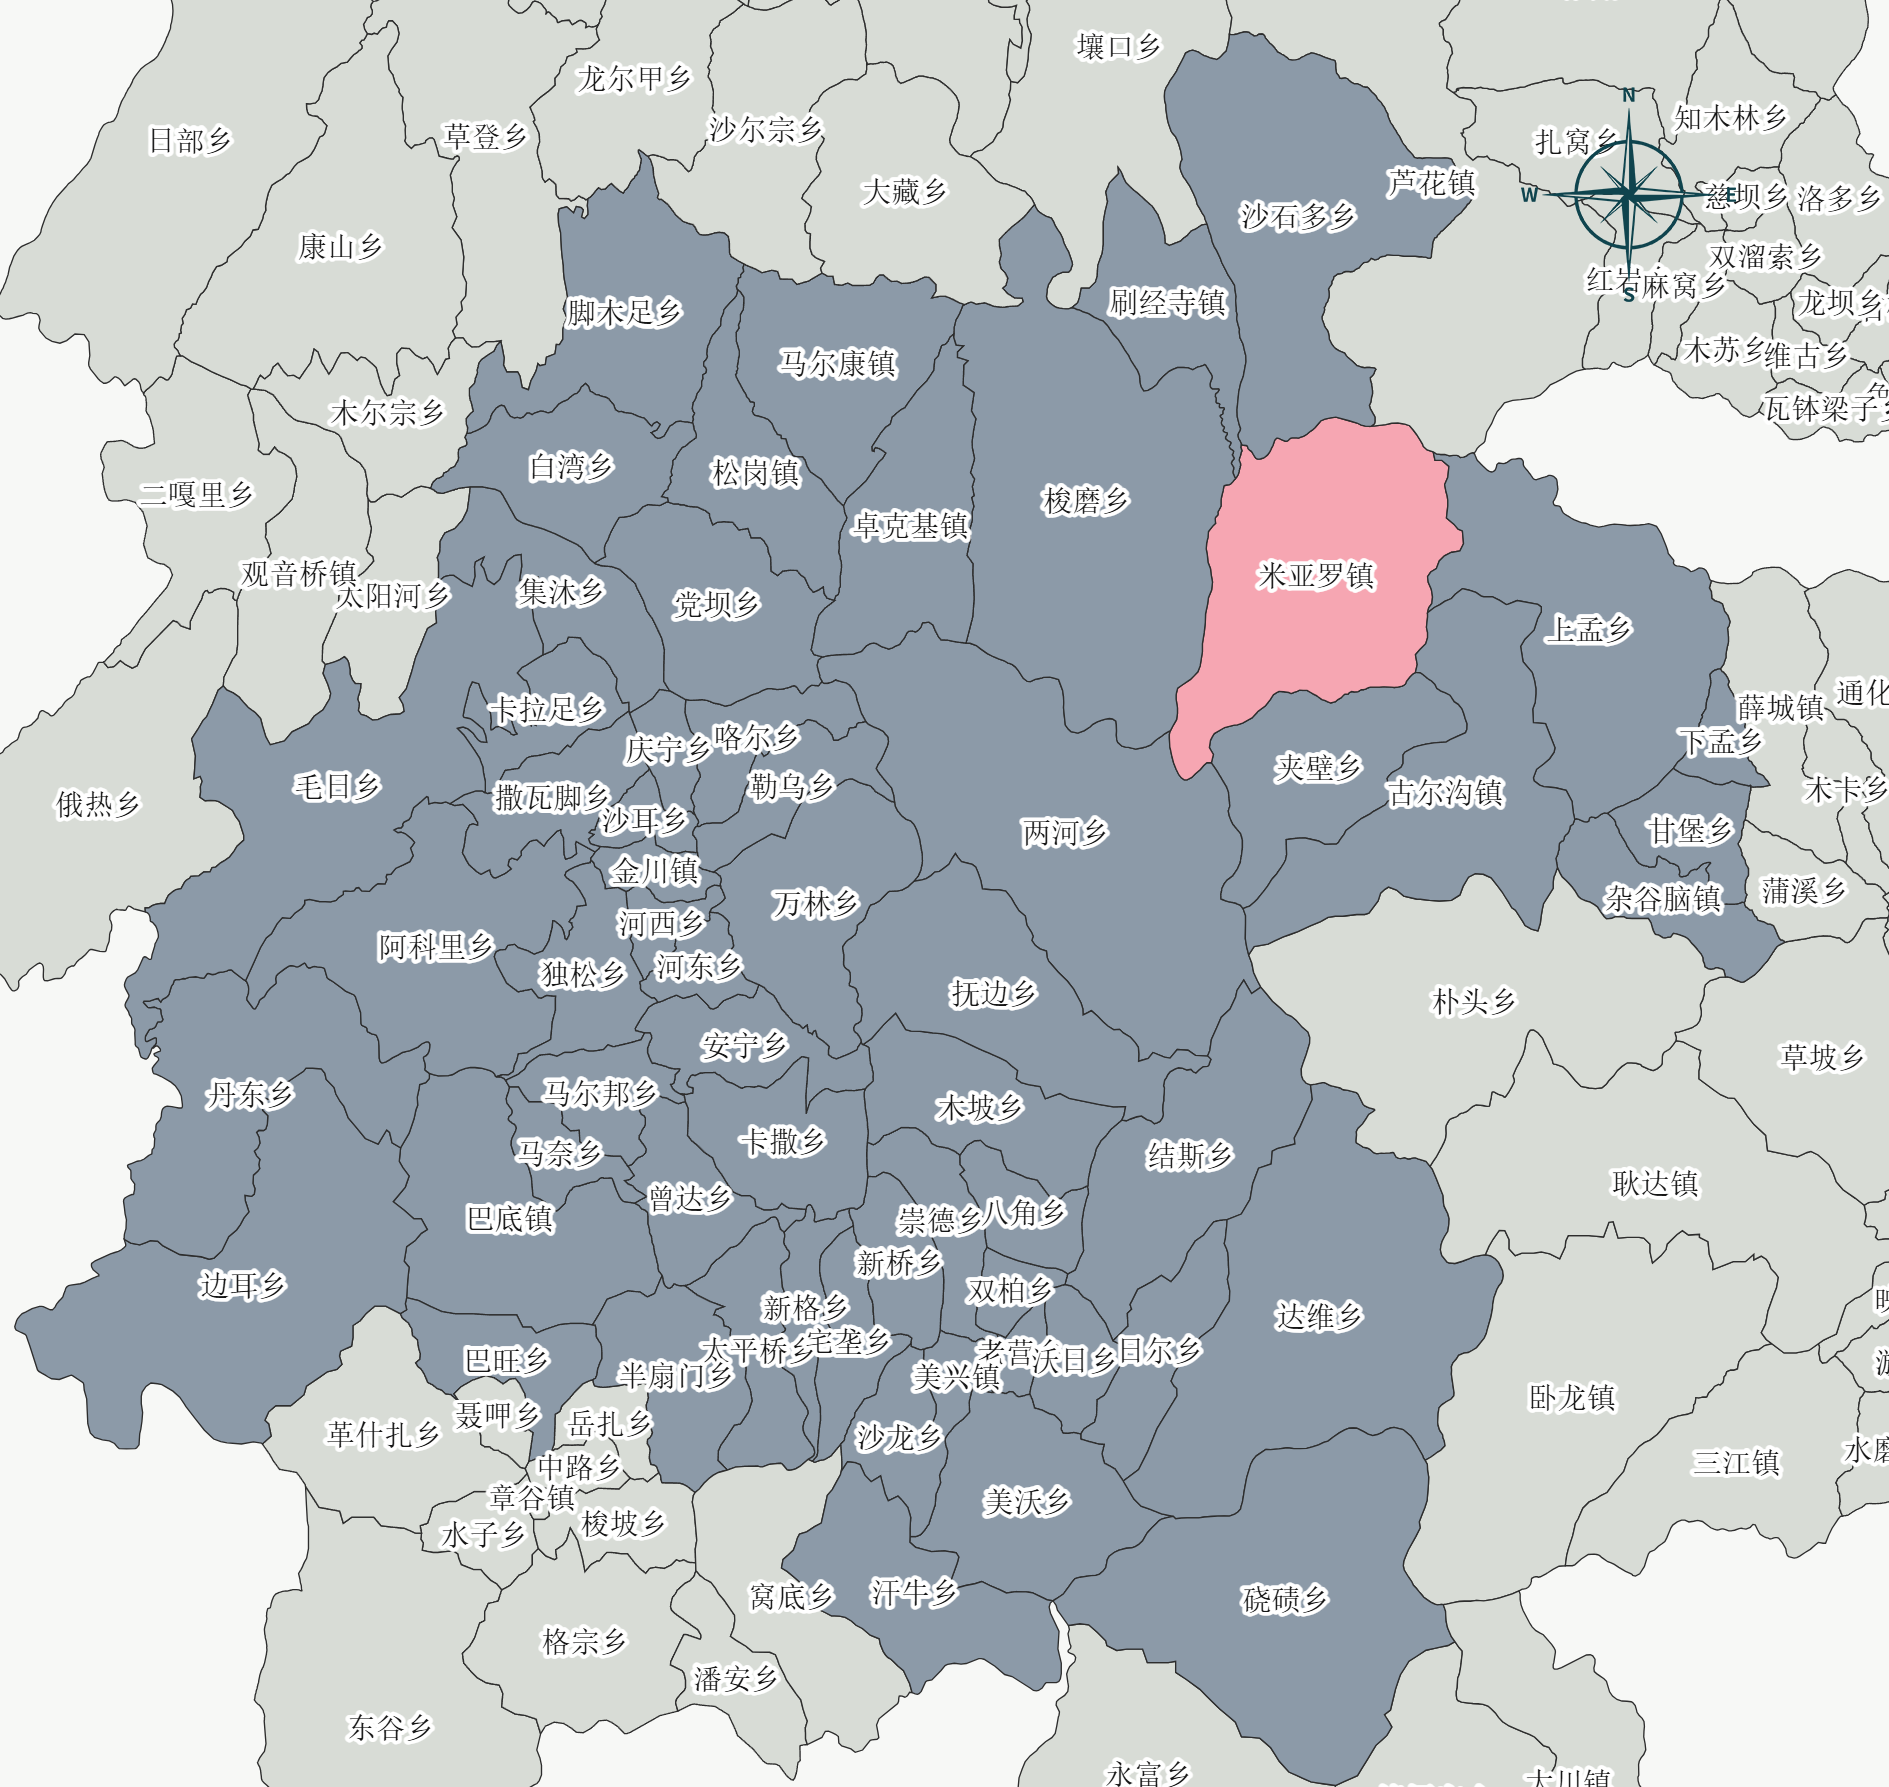
\includegraphics[width=0.8\textwidth]{img/situ.png}
\caption{四土嘉绒语的大致分布}
\label{situ-pic}
\end{figure}

本文所讨论的四土嘉绒语米亚罗话，是四土嘉绒语分布区域东南端的方言之一\cite[102-103]{gates2014situ}。根据\textcite{gates2014situ}的方言学研究，四土嘉绒语可分为中东部和南部方言区。米亚罗话正位于这两个区域的交界处，在民族语言认同和互通度上均表现出过渡性的特征。\textcite{Gong2018-aw}将四土嘉绒语内部方言粗略分为“去鼻冠音”（deprenasalization）类型和“弱化”（leniting）类型，而米亚罗话属于前者。然而，米亚罗话目前仍基本处于文献记录不足状态。现存唯一的记录是一份包含约200个句子和1200个词汇的简短调查，是\textcite{Nagano2013-hy}在嘉绒语组全域进行的大型调查项目的一部分；但这份记录缺乏语音或音系分析。本文将通过田野调查所得材料，首次系统分析四土嘉绒语米亚罗话的音系。

\section{田野工作与语料}

本文的记录对象主要是米亚罗话在理县米亚罗镇的变体。本文的描写基于作者自2025年以来的三次田野调查（2025.1-2、4-5、8-9月）。调查内容包括：对词表进行诱导式调查和录音\footnote{词表参考\textcite{Huang1992,Xiang2008,Lin-2016-dr}进行编制。}、录制故事和对话等长篇语料。除了线下的田野调查，还通过电话、微信等手段与发音人保持联系。本文基于的录音音频数据均为线下录音，录音在安静的室内进行，录音设备为TASCAM DR100mk3录音笔，音频采样率为48 kHz，采样精度为24-bit，保存为立体声WAV格式。录音后的音频文件在Adobe Audition软件中进行剪辑与整理，未进行任何降噪滤波处理。

本文的大部分记音、录音数据及音系分析，均基于主要发音人翁真卓玛（\tib{དབང་འཛིན་སྒྲོལ་མ།}）。发音人出生于1974年，自幼生活在米亚罗镇，现于当地经营一家民宿。其母语为四土嘉绒语米亚罗话，并能流利使用汉语西南官话。此外，她还曾在汶川县就读中专，并学习过一段时间英语。

此外，本文的部分数据有赖于其他发音人。斯玛朗（男，1967年出生）是米亚罗镇米亚罗村的一名猎户，为本文提供了部分动物、植物词汇数据；阿让（男，1938年出生）是米亚罗镇斯博果村的一名农户，为本文提供了部分长语料数据和词汇数据。

本文的记音主要采用国际语音学学会发布的国际音标系统；在此基础上，使用了汉藏语语言学界常使用的/ɿ/标记舌尖前不圆唇元音，相当于国际音标的/ɹ̩/。对于声调，基于四土嘉绒语米亚罗话的词调模式和底层的缺性声调对立（详见第\ref{chaptertone}章），本文在记音中采用两种方式：词末音节韵核为V，或词末标“1”表示“1调”即底层零声调；词末音节韵核为V̂，或词末标“2”表示“2调”即底层降调。

目前，本文涉及的所有词汇的记音和音频数据均已被整理好，并收录、公开在作者开发的嘉绒语词表数据库中，可通过\url{https://flagrain.cn/rgyalrong/}访问。本文涉及的诱导式调查和自然语料的句子音频也已被切分好，可以通过电子邮件me@flagrain.cn向作者取得。

对于文内音频和文本数据的处理，本文均采用作者独立编写的Python程序进行；尤其地，对音频的声学分析采用了Praat的Python接口Parselmouth \parencite{jadoul2018parselmouth,boersma2026praat}。